
\documentclass[tikz,convert={convertexe={magick.exe}}]{standalone}
\usetikzlibrary{snakes}

\begin{document}
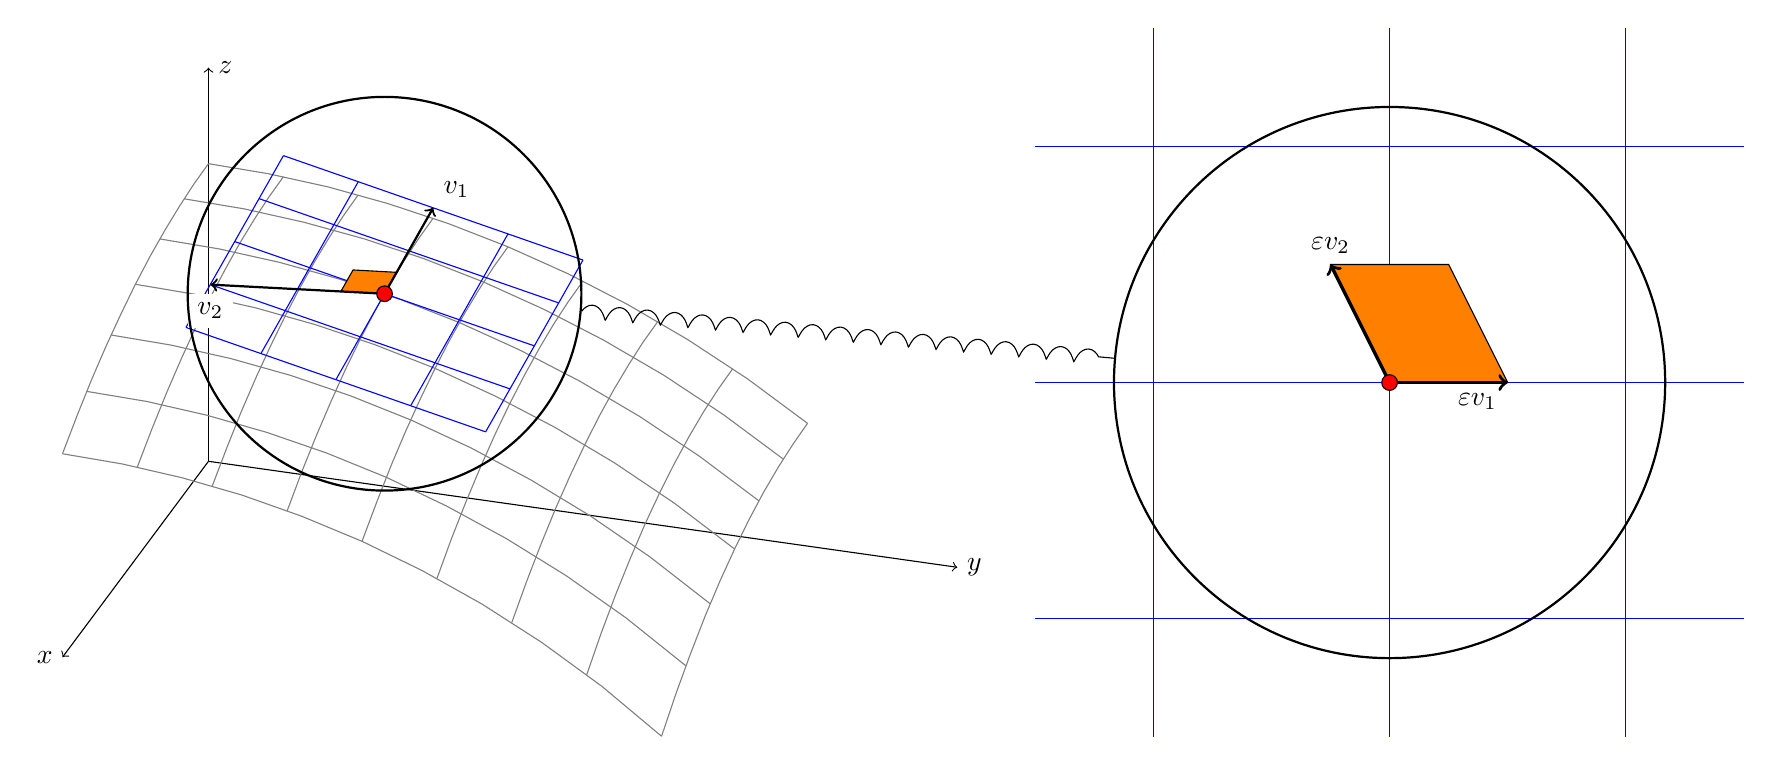
\begin{tikzpicture}

\begin{scope}[scale=2]
\draw[->] (0.000,0.000)--(-0.927,-1.244) node[left] {$x$};
\draw[->] (0.000,0.000)--(4.755,-0.673) node[right] {$y$};
\draw[->] (0.000,0.000)--(0.000,2.5) node[right] {$z$};

\draw[gray] (0.000,1.890)--(0.380,1.826)--(0.761,1.742)--(1.141,1.636)--(1.522,1.510)--(1.902,1.362)--(2.283,1.191)--(2.663,0.995)--(3.043,0.773)--(3.424,0.523)--(3.804,0.241);
\draw[gray] (-0.155,1.667)--(0.226,1.603)--(0.606,1.518)--(0.987,1.413)--(1.367,1.287)--(1.748,1.138)--(2.128,0.966)--(2.508,0.770)--(2.889,0.548)--(3.269,0.297)--(3.650,0.014);
\draw[gray] (-0.309,1.412)--(0.071,1.348)--(0.452,1.263)--(0.832,1.157)--(1.213,1.030)--(1.593,0.881)--(1.974,0.708)--(2.354,0.511)--(2.734,0.287)--(3.115,0.034)--(3.495,-0.251);
\draw[gray] (-0.464,1.124)--(-0.083,1.060)--(0.297,0.975)--(0.678,0.868)--(1.058,0.740)--(1.439,0.590)--(1.819,0.415)--(2.199,0.216)--(2.580,-0.011)--(2.960,-0.267)--(3.341,-0.557);
\draw[gray] (-0.618,0.802)--(-0.238,0.738)--(0.143,0.652)--(0.523,0.545)--(0.904,0.415)--(1.284,0.263)--(1.665,0.086)--(2.045,-0.117)--(2.425,-0.347)--(2.806,-0.609)--(3.186,-0.905);
\draw[gray] (-0.773,0.444)--(-0.392,0.380)--(-0.012,0.293)--(0.369,0.184)--(0.749,0.053)--(1.130,-0.102)--(1.510,-0.283)--(1.890,-0.490)--(2.271,-0.726)--(2.651,-0.994)--(3.032,-1.299);
\draw[gray] (-0.927,0.048)--(-0.547,-0.017)--(-0.166,-0.105)--(0.214,-0.215)--(0.595,-0.350)--(0.975,-0.508)--(1.355,-0.693)--(1.736,-0.906)--(2.116,-1.150)--(2.497,-1.428)--(2.877,-1.746);
\draw[gray] (0.000,1.890)--(-0.093,1.760)--(-0.185,1.618)--(-0.278,1.465)--(-0.371,1.301)--(-0.464,1.124)--(-0.556,0.935)--(-0.649,0.734)--(-0.742,0.519)--(-0.834,0.291)--(-0.927,0.048);
\draw[gray] (0.476,1.807)--(0.383,1.677)--(0.290,1.535)--(0.197,1.382)--(0.105,1.217)--(0.012,1.040)--(-0.081,0.851)--(-0.173,0.650)--(-0.266,0.435)--(-0.359,0.206)--(-0.452,-0.037);
\draw[gray] (0.951,1.692)--(0.858,1.561)--(0.766,1.420)--(0.673,1.266)--(0.580,1.101)--(0.488,0.924)--(0.395,0.734)--(0.302,0.532)--(0.209,0.317)--(0.117,0.087)--(0.024,-0.157);
\draw[gray] (1.427,1.544)--(1.334,1.414)--(1.241,1.272)--(1.148,1.118)--(1.056,0.952)--(0.963,0.774)--(0.870,0.584)--(0.778,0.380)--(0.685,0.163)--(0.592,-0.068)--(0.500,-0.314);
\draw[gray] (1.902,1.362)--(1.809,1.232)--(1.717,1.089)--(1.624,0.935)--(1.531,0.769)--(1.439,0.590)--(1.346,0.398)--(1.253,0.193)--(1.160,-0.026)--(1.068,-0.260)--(0.975,-0.508);
\draw[gray] (2.378,1.144)--(2.285,1.014)--(2.192,0.871)--(2.100,0.716)--(2.007,0.548)--(1.914,0.368)--(1.821,0.174)--(1.729,-0.033)--(1.636,-0.255)--(1.543,-0.491)--(1.451,-0.744);
\draw[gray] (2.853,0.887)--(2.760,0.757)--(2.668,0.613)--(2.575,0.457)--(2.482,0.288)--(2.390,0.106)--(2.297,-0.090)--(2.204,-0.300)--(2.112,-0.525)--(2.019,-0.766)--(1.926,-1.024);
\draw[gray] (3.329,0.588)--(3.236,0.457)--(3.143,0.313)--(3.051,0.156)--(2.958,-0.015)--(2.865,-0.200)--(2.772,-0.399)--(2.680,-0.613)--(2.587,-0.843)--(2.494,-1.090)--(2.402,-1.355);
\draw[gray] (3.804,0.241)--(3.712,0.109)--(3.619,-0.036)--(3.526,-0.195)--(3.433,-0.369)--(3.341,-0.557)--(3.248,-0.760)--(3.155,-0.980)--(3.063,-1.216)--(2.970,-1.471)--(2.877,-1.746);

\draw[blue] (0.476,1.941)--(2.378,1.278);
\draw[blue] (0.321,1.668)--(2.223,1.006);
\draw[blue] (0.167,1.395)--(2.069,0.733);
\draw[blue] (0.012,1.122)--(1.914,0.460);
\draw[blue] (-0.143,0.850)--(1.760,0.187);
\draw[blue] (0.476,1.941)--(-0.143,0.850);
\draw[blue] (0.951,1.775)--(0.333,0.684);
\draw[blue] (1.427,1.610)--(0.809,0.518);
\draw[blue] (1.902,1.444)--(1.284,0.353);
\draw[blue] (2.378,1.278)--(1.760,0.187);


\draw[fill=orange] (1.118,1.064)--(1.195,1.200)--(0.918,1.215)--(0.841,1.079)--cycle;
\draw[->,thick] (1.118,1.064)--(1.427,1.610) node[above right] {$v_1$};
\draw[->,thick] (1.118,1.064)--(0.012,1.122) node[below, yshift=-.1cm,fill=white] {$v_2$};

\node[circle,draw,fill=red,inner sep=2pt] (P) at (1.118,1.064) {};

\node[circle,draw,thick,minimum size=5cm] (Q) at (P) {};
\end{scope}

\begin{scope}[xshift=15cm, yshift=1cm, scale=3]

\foreach \x in {-1,0,1} 
\draw[blue] (\x,-1.5) -- (\x,1.5);
\foreach \y in {-1,0,1} 
\draw[blue] (-1.5,\y) -- (1.5,\y);

\draw[fill=orange] (0,0)--(.5,0)--(.25,.5)--(-.25,.5)--cycle;
\draw[->,very thick] (0,0) -- (.5,0) node[below left] {$\varepsilon v_1$};
\draw[->,very thick] (0,0) -- (-.25,.5) node[above] {$\varepsilon v_2$};

\node[circle,draw,fill=red,inner sep=2pt] (PP) at (0,0) {};
\node[circle,draw,thick,minimum size=7cm] (R) at (PP) {};
\end{scope}

\draw[snake=coil] (Q) -- (R);
\end{tikzpicture}
\end{document}